\documentclass[aps,prd,10pt,onecolumn,nofootinbib,superscriptaddress,floatfix]{revtex4-2}

\usepackage[T1]{fontenc}
\usepackage{lmodern}
\usepackage[utf8]{inputenc}
\input{glyphtounicode}
\pdfgentounicode=1
\usepackage{amsmath,amssymb,mathtools}
\usepackage{bm}
\usepackage{graphicx}
\usepackage{placeins}
\usepackage{hyperref}

\hypersetup{
  colorlinks=true,
  linkcolor=blue,
  citecolor=blue,
  urlcolor=blue
}

\begin{document}
\raggedbottom

\title{Can a Wormhole Induce a Monopole?}

\author{Sergei Slobodov}
\email{sergei@slobodov.com}
\noaffiliation

\date{\today}

\begin{abstract}
Could a body orbiting near one mouth of a traversable wormhole make the mass
seen near the other mouth rise and fall?  We show that the local vacuum
Einstein equations keep the first-order mass monopole constant on a
Schwarzschild background, even for nonspherical source motion.
When spacetime is vacuum sufficiently far from the observer-side mouth,
the asymptotic mass cannot increase even with an evolving throat,
excluding the proposed rise and fall.
Source motion can nevertheless modulate radiative mass loss.
The Maxwell counterpart is exact: without current crossing the measuring
surface, the measured monopole charge remains constant.
The local gravitational and Maxwell results require neither a compact
interior nor an asymptotic end.
\end{abstract}

\maketitle

\section{Introduction}
\label{sec:introduction}

A wormhole can support a static mass at either mouth.  Dai and Stojkovic
(DS) propose that a body orbiting near one mouth makes the mass seen near
the other rise and fall \cite{DaiStojkovic2019Observing}.

In the DS model, two Schwarzschild exteriors are joined at throat radius
$R$, with a mass $\mu$ at radius $A$ in one exterior.  The static
observer-side mass coefficient is $b=\mu R/A$.  Replacing $A$ by $A(t)$
produces the periodically varying $1/r^2$ acceleration also used by
Simonetti et al.~\cite{SimonettiEtAl2021SensitiveSearches} and
Moiseev and Sazhina~\cite{MoiseevSazhina2025ObservationalSearch}.

A family of static solutions need not describe an allowed evolution.
We show that Maxwell charge is exactly conserved without current through
the measuring surface.  In gravity, the first-order mass monopole is
constant in a Schwarzschild vacuum region.  Both results are local and
require neither a compact interior
nor an asymptotic end.

Beyond first order, we use the exact Bondi mass-loss law.  When the observer
end is vacuum near future null infinity, its mass can decrease through
radiation but cannot rise and fall periodically, even with an evolving
throat.  This asymptotic result requires no small-source approximation.

Appendix~\ref{app:separation} constructs a one-ended separated-mouth limit;
Appendix~\ref{app:quadrupole} gives a quasistatic quadrupole benchmark.
We use $G=c=1$ and $r_g=2M$, where $M$ is the background Schwarzschild
mass; only the local Schwarzschild calculation and benchmark assume
$\mu/M\ll1$.

\section{Conservation of electric monopole charge}
\label{sec:maxwell}

In the DS electrostatic model, two flat exteriors are joined at $r=R$,
with charge $q$ at $r_1=A$ in one exterior.  Let $c_1,c_2$ be the
asymptotic potentials.  Matching the potential and its normal derivative
gives the field in the other exterior,
\begin{equation}
 V_2=c_2+\sum_{\ell\ge0}\frac{B_\ell}{r_2^{\ell+1}}
 P_\ell(\cos\theta_2),\qquad
 B_{\ell\ge1}=q\,\frac{2\ell+1}{2(\ell+1)}
 \frac{R^{2\ell+1}}{A^{\ell+1}},\qquad
 B_0=\frac{qR}{2A}+\frac{R}{2}(c_1-c_2).
 \label{eq:ds-multipoles}
\end{equation}
Here $P_\ell$ is a Legendre polynomial and the observer-side charge is
$Q_2=B_0$.  The source position fixes the higher multipoles but not the
monopole, since $c_1-c_2$ is independent boundary data.
DS set $c_1=c_2$, obtaining $Q_2=qR/(2A)$
\cite{DaiStojkovic2019Observing}.

The allowed evolution is fixed by Maxwell's equations.
Let $F$ be the electromagnetic field strength, $j$ the electric current
one-form, and $\star$ the Hodge dual.  On a closed measuring surface $S$,
define
\begin{equation}
 Q[S]=\frac{1}{4\pi}\int_S\star F.
 \label{eq:maxwell-charge}
\end{equation}
A family of such surfaces sweeps out a timelike worldtube $\mathcal T$
with boundary $S_{t_2}-S_{t_1}$.  Integrating $d\star F=4\pi\star j$
and applying Stokes' theorem gives
\begin{equation}
 Q[S_{t_2}]-Q[S_{t_1}]=\int_{\mathcal T}\star j.
 \label{eq:maxwell-balance}
\end{equation}
Without current across $\mathcal T$, the charge is constant.
This is exact even on an evolving metric and requires neither a compact
interior nor an asymptotic end.  Electromagnetic radiation carries
energy, not charge.  Frolov and Novikov established this flux balance
for wormholes \cite{FrolovNovikov1990PhysicalEffects}.
The same local balance applies to a one-ended handle.\footnote{There is
only one asymptotic end.  The flux mode instead permits nonzero circulation
around a loop through the throat and back through the exterior that bounds
no surface \cite{FrolovNovikov1990PhysicalEffects}.}

Imposing $c_1=c_2$ anew as $A$ changes
selects different charges, not successive states of a no-current
evolution.  The charge stays fixed during evolution.  In a quasistatic
description, the potential difference must therefore adjust.
The DS relation $Q_1+Q_2=q$, with $Q_1$ the
source-side flux, conserves the sum;
Eq.~\eqref{eq:maxwell-balance} conserves each charge separately when
neither measuring worldtube is crossed.

Fixed monopole flux does not eliminate the transmitted field.
Figure~\ref{fig:fixed-sector-field} shows the $B_0=0$ solution:
the observer-side field is nonzero but contains only $\ell\ge1$.
The fixed-flux electrostatic problem was developed by Frolov and Novikov,
and by Krasnikov
\cite{FrolovNovikov1990PhysicalEffects,Krasnikov2008ElectrostaticInteraction}.

\begin{figure}[!htbp]
  \centering
  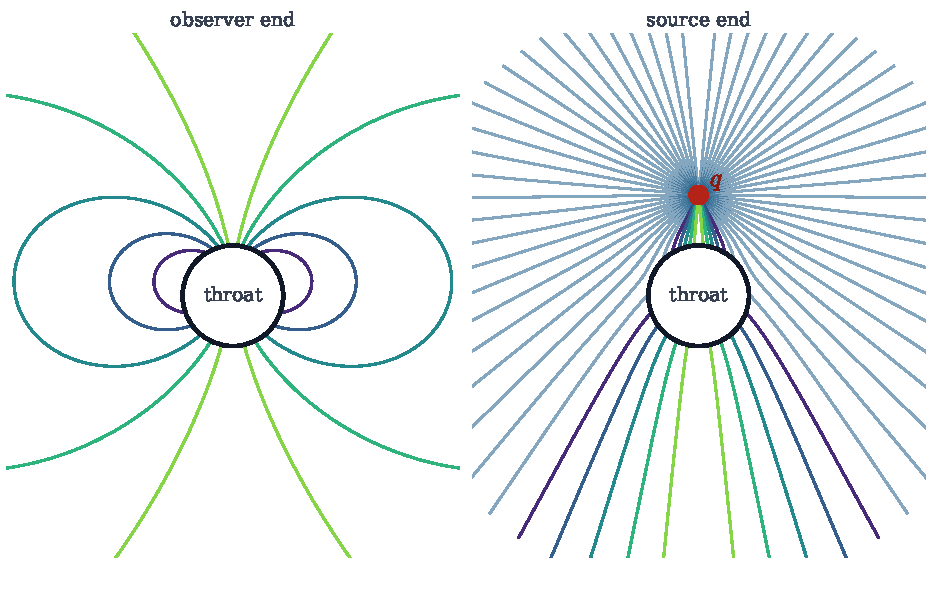
\includegraphics[width=0.82\textwidth]{figures/fig_thinshell_fixed_monopole_flux_v7.pdf}
  \caption{The zero-flux member of Eq.~\eqref{eq:ds-multipoles}: $B_0=0$,
  requiring $c_2-c_1=q/A$.  The black circles represent the same throat sphere
  in the two exterior charts.  Field lines cross the throat but return through
  another angular band, giving zero net flux.  The
  observer-side field is nonzero and contains only $\ell\ge1$ terms.}
  \label{fig:fixed-sector-field}
\end{figure}

\FloatBarrier

\section{Constancy of the first-order mass monopole}
\label{sec:gravity}

In the DS construction the Schwarzschild exteriors have
$d\bar s^2=-f\,dt^2+f^{-1}dr^2+r^2d\Omega^2$, with
$f=1-r_g/r$, and are joined at $R>r_g$.
In their revised preprint, the observer-side static perturbation is
\cite{DaiStojkovic2019ObservingV3}
\begin{equation}
 h^{\mathrm{obs}}_{tt}=\frac{2b}{r_2},\qquad
 h^{\mathrm{obs}}_{rr}=\frac{2br_2}{(r_2-r_g)^2},\qquad
 b=\frac{\mu R}{A}.
 \label{eq:ds-observer-mode}
\end{equation}
Both components give
$h^{\mathrm{obs}}_{\alpha\beta}=b\,\partial_M\bar g_{\alpha\beta}$:
$b$ is a mass shift, with far-field acceleration $-b/r_2^2$, not an
arbitrary potential coefficient.

At first order about Schwarzschild, the harmonic sectors decouple.
The monopole equation therefore applies independently of the source's
nonspherical motion.

\begin{samepage}
Promoting $A$ to $A(t)$ makes this perturbation the linearization of
the metric above with $f$ replaced by
$F(t,r_2)=1-2[M+b(t)]/r_2$.  The linearized mixed Einstein component is
\begin{equation}
 \delta G^r{}_t=\frac{2\dot b}{r_2^2}
 =-\frac{2\mu R\dot A}{A^2r_2^2}.
 \label{eq:momentum-constraint}
\end{equation}
Vacuum therefore requires $\dot b=0$: the proposed monopole modulation
vanishes.  The constant mass shift is fixed by the initial data, not by
the instantaneous orbital radius.
In spherical symmetry, Krasnikov identified this obstruction using
Birkhoff's theorem \cite{Krasnikov2020CommentObserving}.
\end{samepage}

More generally, every vacuum
$\ell=0$ perturbation is a constant mass shift plus a coordinate change
\cite{MartelPoisson2005SchwarzschildPerturbations}.
A time-dependent gauge term cannot supply an observable mass change.
The argument is local to the observer's vacuum region; it assumes
neither vacuum at the throat nor any asymptotic structure.
Higher-multipole fields remain possible, as discussed in
Appendix~\ref{app:quadrupole}.

\section{Nonincrease of the asymptotic mass}
\label{sec:nonlinear}

Gravitational radiation can change the mass beyond first order.  Can this
change reproduce the proposed orbital oscillation?  We first consider a
wormhole with two asymptotic ends, assuming regular Bondi asymptotics and
vacuum near the observer end's future null infinity over the interval
considered.  The source and throat may evolve nonlinearly; no energy
condition on the supporting matter is required.
Appendix~\ref{app:separation} connects this setting to mouths sharing one
exterior by taking their exterior separation to infinity.

In a fixed Bondi
frame with retarded time $u$ and areal radius $r$,
\begin{equation}
 g_{uu}=-1+\frac{2m(u,\Omega)}{r}+O(r^{-2}),\qquad
 E_B(u)=\frac{1}{4\pi}\int_{S^2}m(u,\Omega)\,d\Omega.
 \label{eq:bondi-monopole}
\end{equation}
Here $m$ is the Bondi mass aspect.  Its sphere average $E_B$ is the
mass monopole, giving the angle-independent term $2E_B/r$ in $g_{uu}$.
The expansion is in inverse radius, not in source strength.
For the Schwarzschild mass mode of
Eq.~\eqref{eq:ds-observer-mode}, $E_B=M+b$ at first order.

Define the gravitational-wave news tensor by $N_{AB}=\partial_u C_{AB}$,
with $g_{AB}=r^2q_{AB}+rC_{AB}+O(1)$ and $q^{AB}C_{AB}=0$;
indices are raised using the unit-sphere metric $q_{AB}$.
The exact vacuum Bondi balance is
\cite{BondiVanderBurgMetzner1962Gravitational,Sachs1962Asymptotic,
WaldZoupas2000Conserved}
\begin{equation}
 E_B(u_2)-E_B(u_1)
 =-\frac{1}{32\pi}\int_{u_1}^{u_2}du
    \int_{S^2}N_{AB}N^{AB}\,d\Omega\le0,
 \qquad u_2>u_1.
 \label{eq:bondi-integrated}
\end{equation}
The nonnegative integrand makes $E_B$ nonincreasing.
Equal endpoint masses require no outgoing gravitational radiation between
them, so a nonconstant periodic mass is impossible.
The DS prescription $E_B=M+\mu R/A(u)$ increases as the source approaches
the throat and therefore cannot describe this mass evolution.

Source motion can instead modulate the rate of mass loss, for example
through radiation from an induced deformation of the far mouth.
The balance permits such a response but does not determine its magnitude.
A periodic modulation superposed on secular loss is allowed if the total
mass remains nonincreasing.

For mouths in a shared exterior, the source's ordinary external field
remains present at finite separation.  Appendix~\ref{app:separation}
isolates the mouth-centered asymptotic coefficient in a family with
$r\to\infty$ and $r/D\to0$, where $D$ is exterior mouth separation.
The limiting mass is the observer-end Bondi mass and obeys the same balance.

\section{Conclusion}
\label{sec:conclusion}

Maxwell evolution without current preserves the end charge
exactly; the local gravitational vacuum constraint requires the first-order
mass mode to remain constant.  Beyond that approximation, the asymptotic mass at an
observer end vacuum near null infinity can decrease but cannot rise and
fall periodically.  The DS static family does not describe the proposed
orbital monopole signal.  Higher multipoles and a source-modulated rate
of radiative mass loss remain possible.

\begin{acknowledgments}
The author thanks Ilia Slobodov for helpful discussions.
\end{acknowledgments}

\section*{Artificial Intelligence Use Statement}

The author used OpenAI ChatGPT/Codex and Anthropic Claude as interactive
assistants for brainstorming, mathematical and editorial critique, prose
revision, consistency checks, reference searches, and figure preparation.  All
arguments, calculations, citations, figures, and conclusions were reviewed and
revised by the author, who is solely responsible for the manuscript.

\appendix
\section{A one-ended separated-mouth limit}
\label{app:separation}

We construct a one-ended family whose measured energies approach the
observer-end Bondi mass of a two-ended seed as exterior mouth separation grows.
Take a smooth, globally hyperbolic Einstein--matter solution with
Cauchy surface $\Sigma$, compact initial matter support, and two vacuum
asymptotically Euclidean ends satisfying the hypotheses of
Ref.~\cite{ChruscielCorvinoIsenberg2011NBody}, Theorem~1,
including future-timelike ADM four-momenta.
Assume local existence, geometric uniqueness and causal propagation
for the matter theory, with local constraints compatible with the
retained interior and vacuum exterior, and a regular source and
traversable throat throughout the experiment.\footnote{A distributional thin-shell
model requires its own evolution and uniqueness justification.
Compact initial matter support alone does not establish the vacuum
null infinity assumed in Sec.~\ref{sec:nonlinear}.}

For a compact spacetime neighborhood $K$ to the future of $\Sigma$,
retain a connected compact region $P$ containing the source, throat and
the compact initial footprint $J^-(K)\cap\Sigma$ with a margin,
including paths through either mouth.  Choose its two outer boundaries
in the vacuum ends.  The gluing theorem supplies a common one-ended
vacuum exterior matching open collars of both boundaries at arbitrarily
large exterior separation $D$, while leaving $P$ unchanged.
Exact matching preserves the constraints without a shell; causal
geometric uniqueness preserves an isometric copy of $K$ in the
development \cite{Sbierski2015CauchyDevelopment}.

To compare masses, use the Hawking energy of a spacelike two-sphere
with mean-curvature vector $H^a$,
\begin{equation}
 E_H(S)=\sqrt{\frac{|S|}{16\pi}}
 \left(1-\frac{1}{16\pi}\int_S H^aH_a\,dA\right).
 \label{eq:hawking-energy}
\end{equation}
This depends on the geometry at $S$, without a compact physical interior.
Fix a compact retarded-time interval $I$ at the original solution's
observer end, with the vacuum asymptotics of Sec.~\ref{sec:nonlinear}.
Assume outgoing, asymptotically round cuts $S(u,r)$ whose Hawking energies
tend to $E_B(u)$ \cite{MarsSoria2015HawkingEnergy}.
We require this convergence to be uniform on $I$.

Choose $\epsilon_n\to0$ and $r_n\to\infty$ so that the seed energies
approximate $E_B$ within $\epsilon_n$ uniformly on $I$.
For each $n$, preserve the complete initial causal footprint of a
neighborhood of these cuts and the relevant source and throat histories,
then glue outside it with $D_n>nr_n$.  The image cuts $S_n(u)$ have
isometric spacetime neighborhoods, so
\begin{equation}
 \begin{split}
 E_n(u)&:=E_H(S_n(u))=E_H(S(u,r_n)),\\
 \sup_{u\in I}|E_n(u)-E_B(u)|&<\epsilon_n,
 \qquad r_n/D_n\longrightarrow0.
 \end{split}
 \label{eq:handle-energy-limit}
\end{equation}
The time labels come from the seed.  Although measurement times grow
with $r_n$ at fixed $u$, their complete causal footprints were protected
before gluing.  For $u_1<u_2$ in $I$,
\begin{equation}
 E_n(u_2)-E_n(u_1)
 \le E_B(u_2)-E_B(u_1)+2\epsilon_n
 \le2\epsilon_n.
 \label{eq:handle-no-rise}
\end{equation}
The construction needs no uniform all-time stability estimate and
asserts no universal finite-$D$ correction law.
No upward excursion of finite amplitude survives this limit.

\newpage
\section{A quasistatic quadrupole benchmark}
\label{app:quadrupole}

We estimate the quasistatic tidal response as the source moves.  At first
order about Schwarzschild, the even-parity $\ell=1$ vacuum mode is a
locally pure-gauge displacement; the odd-parity mode is a constant
angular-momentum shift \cite{MartelPoisson2005SchwarzschildPerturbations}.
The first local, gauge-invariant time-dependent vacuum field is therefore
quadrupolar \cite{Thorne1980Multipole}, unlike the Maxwell dipole in
Fig.~\ref{fig:fixed-sector-field}.

We compare its quasistatic acceleration with the proposed monopole scale
$a_{\mathrm{DS}}\sim\mu R/(Ar_2^2)$.
In the tidal approximation, the quadrupolar part of the source potential
at the throat scales as $\mu R^2/A^3$, and the transmitted potential
decays as $(R/r_2)^3$.
Radial differentiation therefore gives
\begin{equation}
 \frac{a_2}{a_{\mathrm{DS}}}
 \sim C_2\left(\frac{R}{A}\right)^2
          \left(\frac{R}{r_2}\right)^2.
 \label{eq:quadrupole-benchmark}
\end{equation}
To calculate $C_2$, use the static stiff-shell construction of
Ref.~\cite[Appendix~D.1]{CardosoEtAl2017LoveNumbers}.  Its polar metric
amplitudes on the source and observer sides are
$H_0^{(s)}=\alpha P_2^2(x)+\beta Q_2^2(x)$ and
$H_0^{(o)}=\gamma Q_2^2(x)$, where $x=r/M-1$; no applied tide is present
on the observer side.  With the surface-density perturbation set to zero,
the angular metric amplitude $K$ and its derivative along the continuous
tortoise coordinate are continuous at the throat.  Equivalently,
\begin{equation}
 \frac{\gamma}{\alpha}
 =\frac12\left(\frac{K_P}{K_Q}-\frac{K_P'}{K_Q'}\right)_{r=R},
 \qquad
 C_2=\frac85\left(\frac{M}{R}\right)^5\frac{\gamma}{\alpha}.
 \label{eq:quadrupole-transfer}
\end{equation}
Here $K_P,K_Q$ follow from the cited relation between $K$ and $H_0$ by
inserting $P_2^2,Q_2^2$, respectively; primes denote outward $r$ derivatives.
The normalization follows from $P_2^2(x)\sim3x^2$,
$Q_2^2(x)\sim8/(5x^3)$ and the factor three from radial differentiation.
This gives $0<C_2<5/2$ for $R>2M$, approaching $5/2$ in the weak-field
limit and zero as $R\to2M$.

For the favorable Sgr~A*/S2 benchmark $A\sim R\sim r_g$,
$r_g\simeq0.084\,\mathrm{AU}$ and $r_2\simeq1000\,\mathrm{AU}$,
the geometric factor in Eq.~\eqref{eq:quadrupole-benchmark} is
$7\times10^{-9}$, giving an upper scale of order $10^{-8}$.
The near-mouth substitution is an order-of-magnitude extrapolation of
the tidal scaling, not an exact orbital calculation.
We retain $R-r_g\gg\mu$ for perturbative consistency.
This static-response estimate is not a bound on radiation from a
dynamical throat.

\bibliographystyle{apsrev4-2}
\bibliography{references,references_v10_additions}

\end{document}
